\chapter{Arhitectura aplicației}

În mare parte aplicația este construită în jurul unei singure scene folosind $Unity$, arhitectura aplicației depinzând în mare parte de uneltele disponibile în motorul grafic și modul în care acesta funcționează. Am încercat să împart căt de mult se poate aplicația în module cu o coeziune căt mai ridicată. De acceea sistemul de instanțiere, generare și amplasare a obiectelor este construit cu principalul scop de a fi modular. Chiar și librăria ce modelează prototipul Markov cu stări invizibile este decuplat de algoritmul de antrenare în sine, putând fi schimbat oricând fără a afecta funcționalitatea librăriei.\par

Aplicația folosește și multe funcții de $callback$ pentru a determina cănd anumite elemente din cadrul jocului ar trebui activate. Spre exemplu cea mai folosită funcție este cea de $OnTriggerEnter$, ce determină când un $RigidBody$\footnote{Componenta ce determina daca obiectul este supus motorului de fizica} se intersectează cu un \textit{Box}\textit{Collider}\footnote{Componenta ce determina zona de coliziune a unui obiect}.\par

\begin{lstlisting}[caption=Exemplu de utilizare a functiei OnTriggerEnter]
void OnTriggerEnter(Collider collidingObject){
        if (!this.triggered){
            this.callbackObject.GetComponent<PlatformBuilder>().InstantiatePlatform();
            this.triggered = true;
        }
}
\end{lstlisting}
\par

De asemena $Unity$ dispune de o unealtă foarte utilă numită $Inspector$ ce permite asignarea de referințe a obiectelor din scenă în scripturi, lucru foarte util și eficient atunci cănd este necesară legarea anumitor module. De exemplu $callbackObject$ reprezintă obiectul din scenă de care este atașat codul sursă ce se ocupă de construirea platformelor, numit sugestiv $PlatformBuilder$, din care se apelează funcția $InstantiatePlatform$ destinată acestui scop.\par

\section{Detalii legate de implementarea librăriei}

Cum menționam și anterior pentru implementare am avut nevoie de o librărie ce se ocupă cu calcul numeric. Am folosit $Math.NET$ pentru calculul matriceal și a normelor $L^{2}$, împreună cu structurile speciale $Matrix$ și $Vector$ din cadrul librăriei pentru a manipula parametri $\lambda = \{\textbf{A},\textbf{B},\pi\}$ ai modelului.\par

În cadrul librăriei ce descrie modelul Markov cu stări invizibile s-au folosit o multitudine de funcții auxiliare ce ajută la normalizare și structurarea mai bună a codului. Mai jost sunt prezentate cele mai importante funcții auxiliare din cadrul acesteia.\par

\begin{lstlisting}[caption=Funcție auxiliara ce realizează normalizarea]
private Matrix<double> Normalize(Matrix<double> target, Vector<double> divisors, string mode){
        Matrix<double> output = Matrix<double>.Build.DenseOfMatrix(target);
        for (int i = 0; i < target.RowCount; ++i){
            for (int j = 0; j < target.ColumnCount; ++j){
                if (mode == "row")
                    output[i, j] /= divisors[i];
                if (mode == "column")
                    output[i, j] /= divisors[j];
            }
        }
        return output;
}
\end{lstlisting}


\begin{lstlisting}[caption=Funcție auxiliara ce construiește matricea de frecvență $C$]
private Matrix<double> GetOccurenceMatrix(List<int> observations){
        Matrix<double> occurences = Matrix<double>.Build.Dense(this.emissionCount, this.emissionCount);
        for (int i = 0; i < observations.Count - 1; ++i){
            occurences[observations[i], observations[i + 1]] += 1;
        }
        return occurences;
}
\end{lstlisting}

\begin{lstlisting}[caption=Funcție auxiliara ce contruieste o matrice cu intrări random]
private void SetRandomMatrix(double[,] matrix){
        double[] divisors = new double[matrix.GetLength(0)];
        double rowMax = 0.0f;
        for (int i = 0; i < matrix.GetLength(0); ++i){
            rowMax = 0;
            for (int j = 0; j < matrix.GetLength(1); ++j){
                matrix[i, j] = Random.Range(0.0f, 100.0f);
                rowMax += matrix[i, j];
            }
            divisors[i] = rowMax;
        }
        Normalize(matrix, divisors);
}
\end{lstlisting}
\clearpage

Legat de aplicarea capitoluilui teoretic, antrenarea este realizată de o singură funcție căreia îi sunt pasați parametri modelului, împreună cu secvența de etichete observate. Funcția aplică ecuațiile discutate în cadrul capitolului de aspecte teoretice, bineînțeles adaptate la limbajul de programare folosit.\par

\begin{lstlisting}[caption=Implementare algoritmului de antrenare a modelului]
public double Train(List<int> observations, double[,] transitionProbabilities, double[,] emissionProbabilities, List<double> pi){
        this.SetEmissionMatrix(emissionProbabilities);
        this.SetTransitionMatrix(transitionProbabilities);
        this.SetDrawProbabilities(pi);
        Matrix<double> previousJoinDistribution = Matrix<double>.Build.Dense(this.emissionCount, this.emissionCount);
        Matrix<double> previousEmission = Matrix<double>.Build.Dense(this.stateCount, this.emissionCount);
        Matrix<double> previousTransition = Matrix<double>.Build.Dense(this.stateCount, this.stateCount);
        Matrix<double> jointDistribution;
        Matrix<double> emissionDelta;
        Matrix<double> transitionDelta;
        Matrix<double> occurenceMatrix = this.GetOccurenceMatrix(observations);
        this.SetMatrixBar();
        this.emissionMatrix = this.emissionMatrix.Transpose();
        previousEmission = previousEmission.Transpose();
        double likelihood = 0.0f;
        for (int i = 0; i < this.maxIterations; ++i){
            jointDistribution = occurenceMatrix.PointwiseDivide(this.emissionMatrix.Multiply(this.transitionMatrix).Multiply(this.emissionMatrix.Transpose()));
            transitionDelta = this.transitionMatrix.PointwiseMultiply(this.emissionMatrix.Transpose().Multiply(jointDistribution).Multiply(this.emissionMatrix));
            emissionDelta = this.emissionMatrix.PointwiseMultiply(jointDistribution.Multiply(this.emissionMatrix).Multiply(this.transitionMatrix.Transpose()).Add(jointDistribution.Transpose().Multiply(this.emissionMatrix).Multiply(this.transitionMatrix)));
            this.transitionMatrix = transitionDelta.Divide(transitionDelta.RowSums().Sum());
            this.emissionMatrix = Normalize(emissionDelta, emissionDelta.ColumnSums(), "column");
            if (this.transitionMatrix.Subtract(previousTransition).L2Norm() < this.epsilon && this.emissionMatrix.Subtract(previousEmission).L2Norm() < this.epsilon && jointDistribution.Subtract(previousJoinDistribution).L2Norm() < this.epsilon)
                break;
            previousEmission = emissionMatrix;
            previousTransition = transitionMatrix;
            previousJoinDistribution = jointDistribution;
        }
        likelihood = GetLikelihood(occurenceMatrix, this.transitionMatrix, this.emissionMatrix.Transpose(), this.emissionMatrix.Multiply(this.transitionMatrix).Multiply(this.emissionMatrix.Transpose()));
        this.transitionMatrix = Normalize(this.transitionMatrix, this.transitionMatrix.RowSums(), "row");
        this.emissionMatrix = this.emissionMatrix.Transpose();
        return likelihood;
}
\end{lstlisting}

Funcția $Train$ descrisă mai sus este folosită în clasa mare denumită sugestiv $HMM$ pentru a antrena modelul. Modul cum funcționează $Unity$ toate clasele ce sunt derivate din $MonoBehaviour$ pot fi atașate pe un obiect din scenă. De accea există un obiect ascuns în scenă ce are atașat toți generatorii, putănd schimba foarte ușor toți parametri modelului chiar din $Inspector$. Din cauza acestui lucru librăria este foarte ușor de preluat și utilizat, aceasta conținând și un modul de salvare/citire a parametrilor modelului.\par

În continuare se va prezenta o diagramă $UML$ ce descrie librăria și relația dintre componentele ei. Se poate observa că modelul Markov cu stări invizibile poate lucra complet independent de algoritmul de învățare automată.\par

\vspace{10mm}
\begin{figure}[H]
\centering
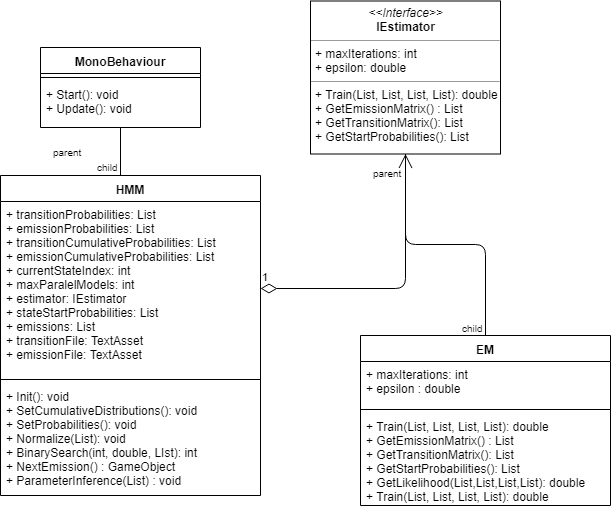
\includegraphics[width=0.75\linewidth]{HMM.png} \par
\caption{Diagrama UML ce modelează libraria de HMM}
\end{figure}

\textit{IEstimator} este interfața ce specifică ce proprietăți și metode algortimul de estimare are nevoie să implementeze. Se observă din schemă implementare modelului $Strategy$, ce elimină asocierea dintre clasa \textit{HMM} și algoritmul de antrenare. Din această cauză se poate face foarte ușor schimbarea algoritmului de antrenare în timpul rulării programului în funcție de necesitate.\par

\begin{lstlisting}[caption=Folosirea funcție $Train$ în cadrul modelului]
public void ParameterInference(List<int> observations)
{
        double[,] bestEmission = this.emissionProbabilities;
        double[,] bestTransition = this.transitionProbabilities;
        double[] startProbabilites = this.stateStartProbabilities.ToArray();
        double maxLoglikelihood = double.MinValue;
        for (int i = 0; i < this.maxParalelModels; ++i){
            double likelihood = estimator.Train(observations, this.transitionProbabilities, this.emissionProbabilities, this.stateStartProbabilities);
            if (maxLoglikelihood < likelihood){
                maxLoglikelihood = likelihood;
                bestEmission = estimator.GetEmissionMatrix();
                bestTransition = estimator.GetTransitionMatrix();
                startProbabilites = estimator.GetStartProbabilities();
            }
            this.SetRandomProbabilities();
        }
        this.emissionProbabilities = bestEmission;
        this.transitionProbabilities = bestTransition;
        this.stateStartProbabilities = new List<double>(startProbabilites);
        this.currentStateIndex = this.SetInitialState();
        this.SetCumulativeDistributions();
    }
}
\end{lstlisting}

\vspace{10mm}
\begin{figure}[H]
\centering
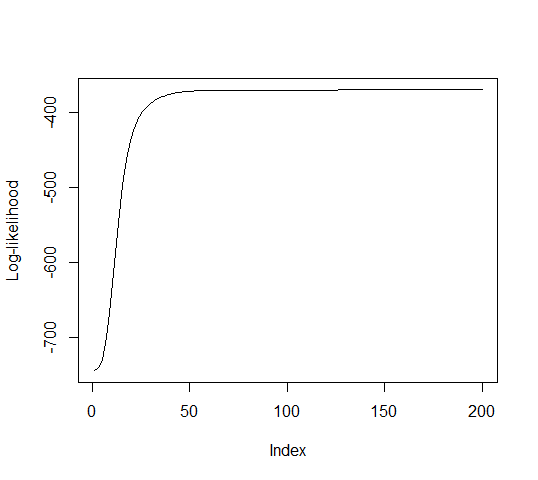
\includegraphics[width=0.75\linewidth]{Learning.png} \par
\caption{Grafic ce arată antrenarea unui generator}
\end{figure}



\section{Detalii legate de implementarea sistemului de instanțiere}

Așa cum am mai menționat modelul Markov cu stări invizibile este folosit ca și generator iar pentru instanțiere a fost necesară implementarea unui sistem ce folosește puncte de $spawn$ amplasate pe platforme. Odată cu aceste puncte există și un script ce descrie dacă punctul de instanțiere poate să conțină mai multe obiecte sau nu, amplasarea lor facandu-se unu după altul. Se poate specifica și rotația obiectului, dar in general se urmarește ca obiectele de pe platformă să fie orientate înspre jucător, în sensul acelor de ceasornic.\par

\vspace{10mm}
\begin{figure}[H]
\centering
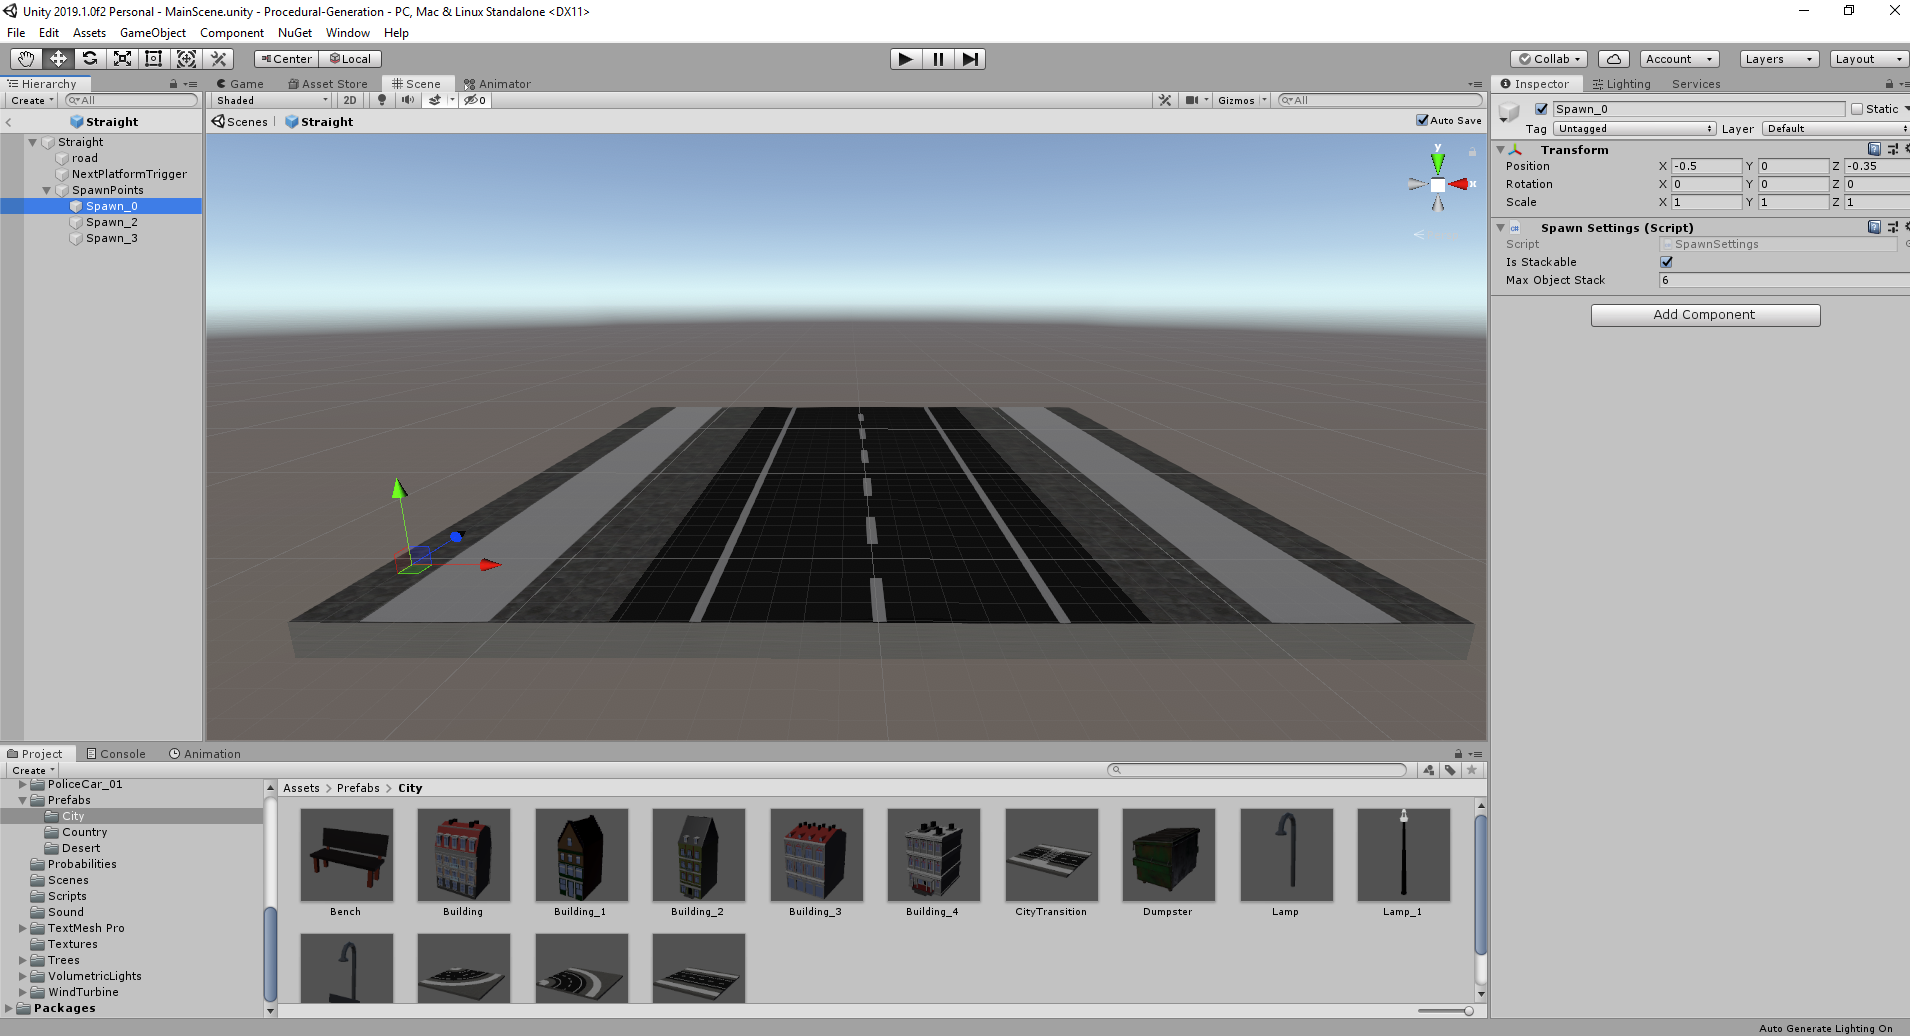
\includegraphics[width=\linewidth]{Spawn.png} \par
\caption{Sistemul de instanțiere}
\end{figure}

De asemenea punctele de $spawn$ sunt plasate exact pe marginea platformei iar algoritmul de instanțiere ia în calcul acest lucru. Cu toate acestea ele pot fi mutate spre interiorul platformei pentru a da senzația de realism. O limitare a acestui sistem este sensibilitatea la numărul de obiecte pe un loc de instanțiere, deoarece acesta nu ține cont de lungimea platformei.

\section{Utilizarea librăriei în joc}

În dezvoltarea acestei librării obiectivele principale au fost modularitatea și usurința de utilizare. Acest lucru a fost realizat foarte simplu datorită modului în care $Unity$ permite atașarea de fișiere sursă pe obiecte din scenă, avănd la dispoziție toti parametri disponibili din acea clasă.\par

\vspace{10mm}
\begin{figure}[H]
\centering
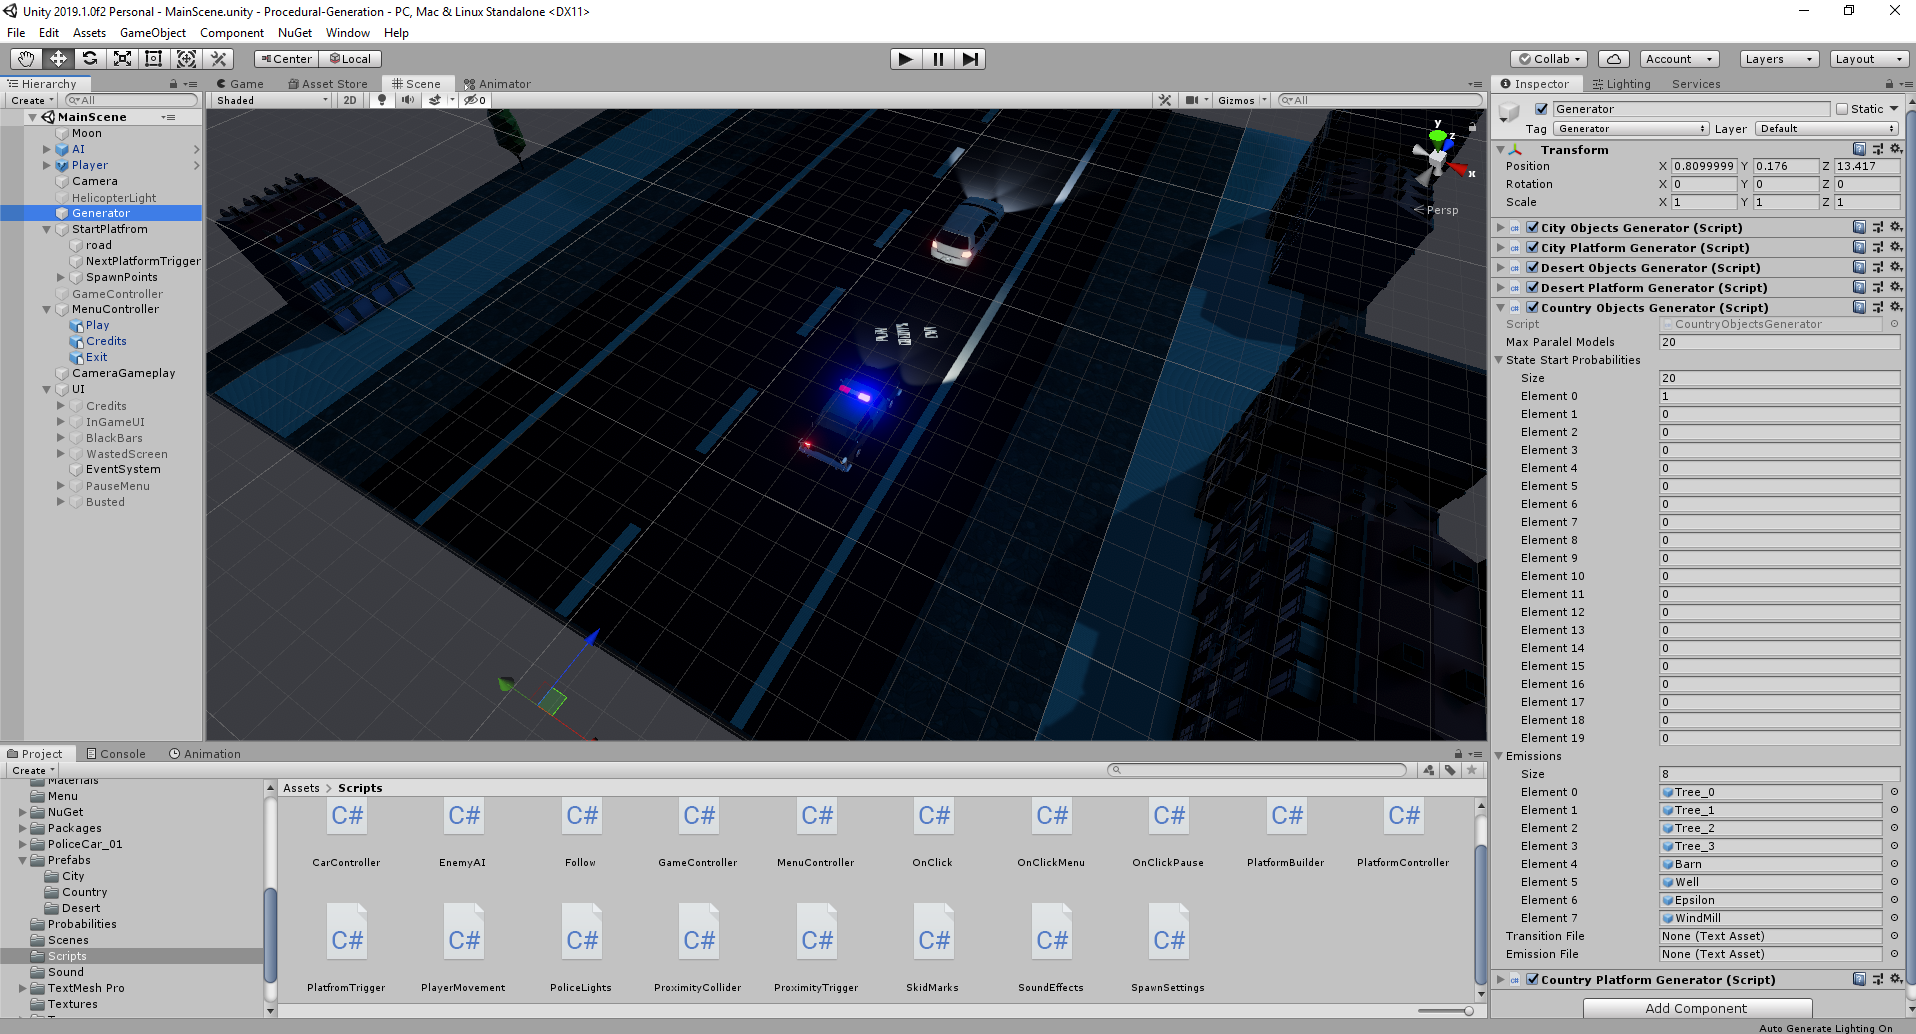
\includegraphics[width=\linewidth]{Generator.png} \par
\caption{Generatorii folosiți în cadrul jocului}
\end{figure}

În general pentru a putea folosi librăria, se definește o clasă nouă ce moștenește din clasa $HMM$, în cadrul careia se apelează funcția $Init()$ în funcția $Start()$.\par

\begin{lstlisting}[caption=Exemplu de folosire a librăriei]
public class DesertObjectsGenerator : HMM{
    void Start(){
        this.Init();
    }
}
\end{lstlisting}

Este necesară această procedură din cauza modului cum functionează $Unity$, deoarece scripturile nu pot fi atașate pe obiecte în cadrul scenei dacă nu sunt derivate din $MonoBehaviour$ iar $C\#$ nu permite moștenirea multiplă.\par

Acest lucru face un pic incomodă folosirea librăriei dar capabilitatea de a putea atașa scriptul de orice obiect din scenă și de a putea adăuga referințe direct din $Inspector$ este mult prea importantă pentru a nu deriva din clasa $MonoBehaviour$.\par

Librăria dispune și de o modalitate persistentă de încarcare e parametrilor unui model și anume prin așa numitele obiecte $TextAsset$ disponibile în cadrul motorului de joc. De exemplu, după antrenarea modelului parametri acestuia pot fi salvați prin apelarea unei funcții într-un astfel de obiect ce poate fi ulterior referențiat librăriei pentru a putea încărca modelul.\par

\section{Detalii legate de aspectul aplicației}

Un alt aspect ce a necesitat destul de mult timp în cadrul acestei aplicații a fost partea de $UI$\footnote{User Interface} căt și îmbunătățirile grafice aduse prin postprocesare, $SSR$, reflecții în timp real, anti-aliasing, bloom, lumină volumetrică și corectare de culoare.\par

\vspace{10mm}
\begin{figure}[H]
\centering
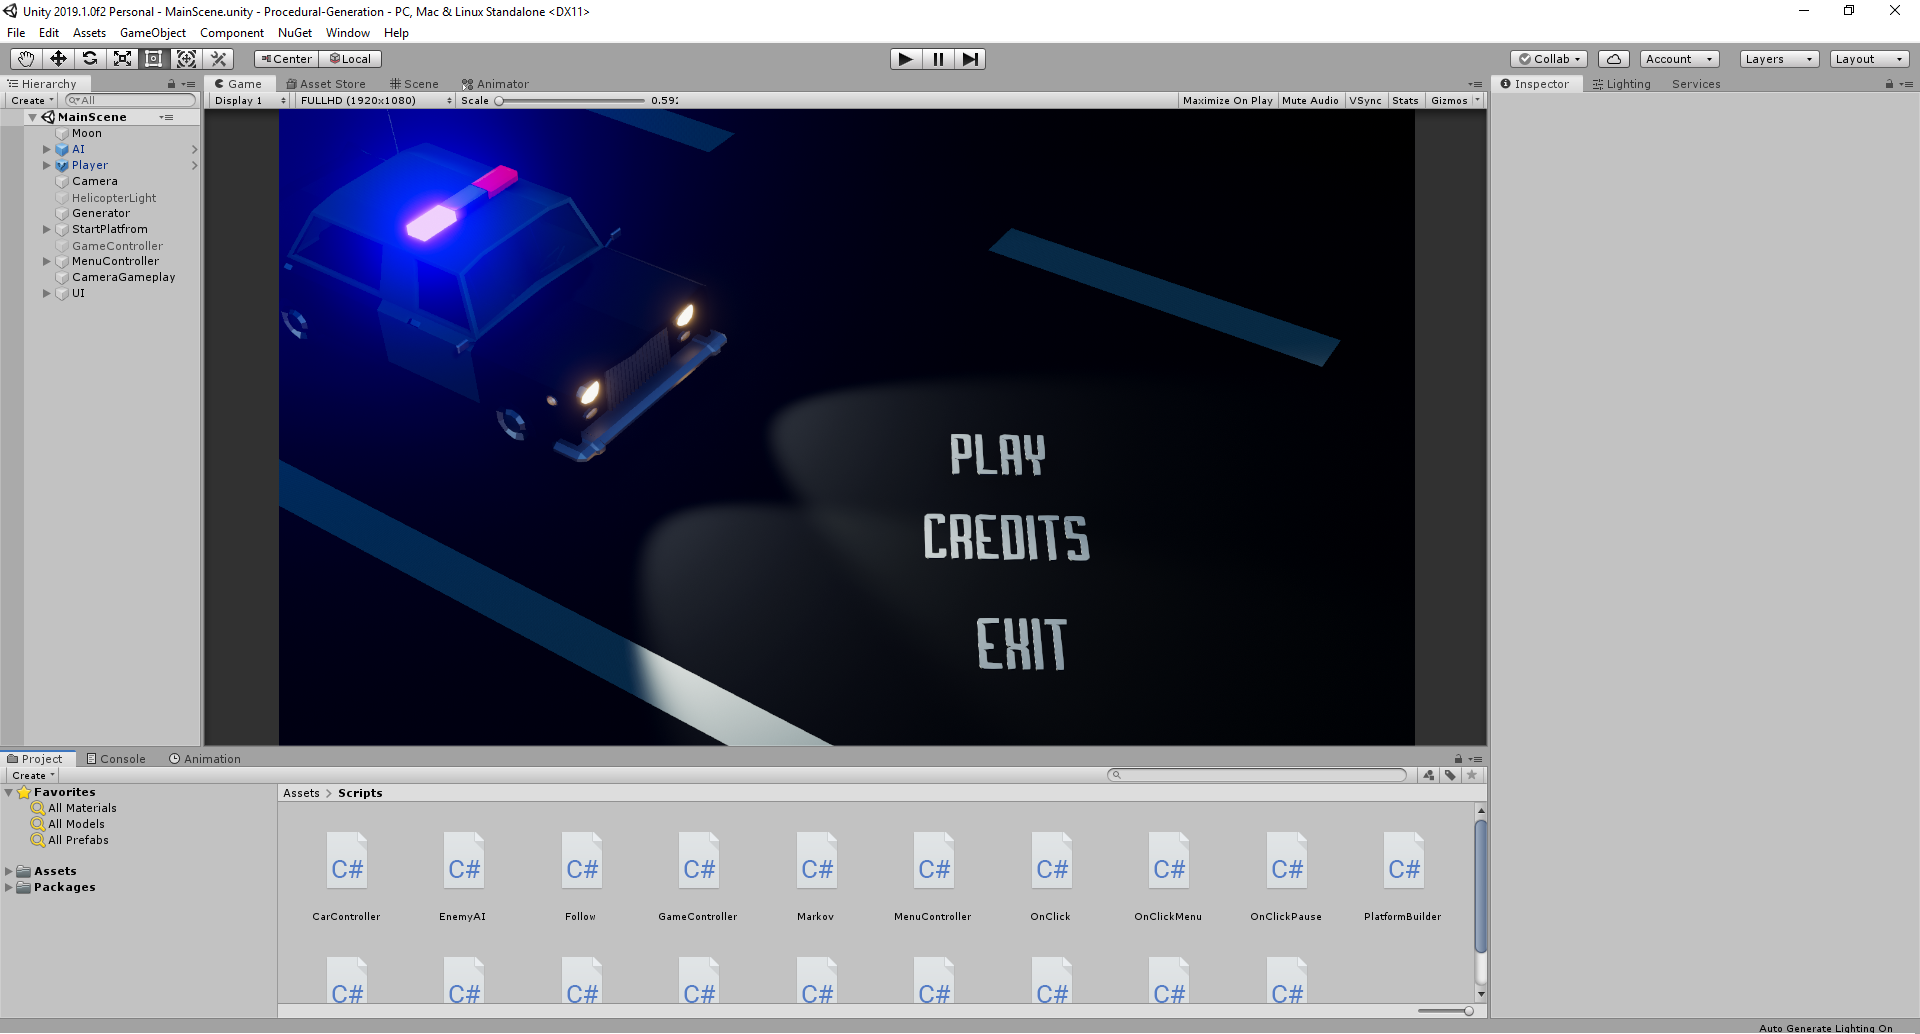
\includegraphics[width=\linewidth]{Unity.png} \par
\caption{Motorul Grafic Unity}
\end{figure}

Pe lângă partea grafică am încercat să adaug animații  atâr obiectelor din cadrul scenei căt și a butoanelor cu care înteracționează jucătorul. Datorită uneltelor din $Unity$ acest lucru a fost ușor de realizat. Pe lângă crearea animațiilor am fost nevoit să utilizez și un automat cu stări finite, unde fiecare nod reprezintă de fapt o altă animație. În $Unity$ acestă unealtă se numește $Animator$, și manipulează condițiile de trece de la o stare la altă și durata.\par

\vspace{10mm}
\begin{figure}[H]
\centering
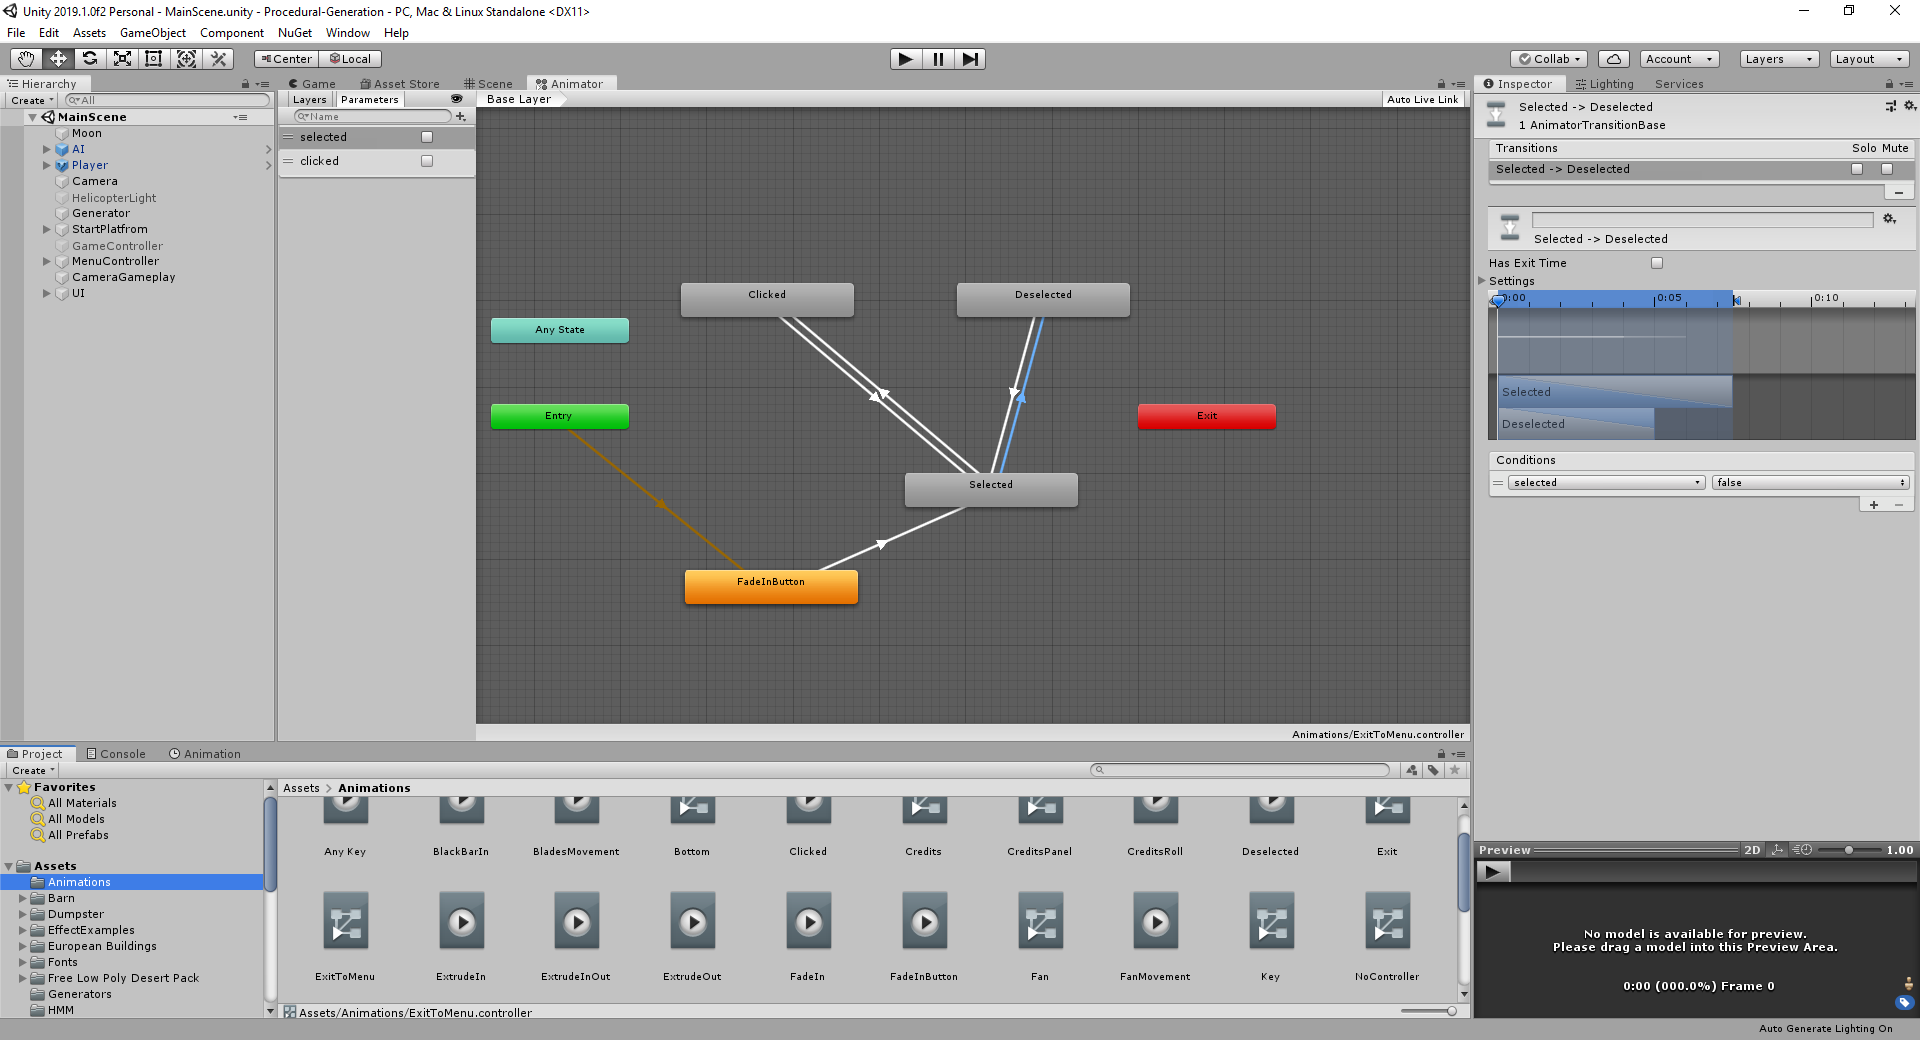
\includegraphics[width=\linewidth]{Animator.png} \par
\caption{Utilitarul folosit pentru animații}
\end{figure}

Am încercat în mare parte să refolosesc animații și obiecte din motive de eficiență și spațiu de stocare. De acceea multe stări din automatele de animații se repetă. Pentru controlul acțiunii butoanelor din meniuri, comportamentul s-a modelat folosind funcții ce sunt apelate la ieșirea din stare, mai exact la terminarea animației.\par

\begin{lstlisting}[caption=Exemplu de folosire a evenimentului $OnStateExit$]
override public void OnStateExit(Animator animator, AnimatorStateInfo stateInfo, int layerIndex)
{
        MenuController controller = GameObject.FindGameObjectWithTag("MenuController").GetComponent<MenuController>();
        switch (animator.name){
            case "Play":
                controller.OnGameStart();
                break;
            case "Credits":
                controller.OnCredits();
                break;
            case "Exit":
                controller.OnGameExit();
                break;
            default:
                break;
        }
}
\end{lstlisting}

Jocul dispune de un meniu principal, unu de pauză în timpul jocului și unul ce anunță sfărșitul jocului. Mai jos sunt prezentate aceste trei meniuri, împreună cu opțiunile lor.\par

\vspace{10mm}
\begin{figure}[H]
\centering
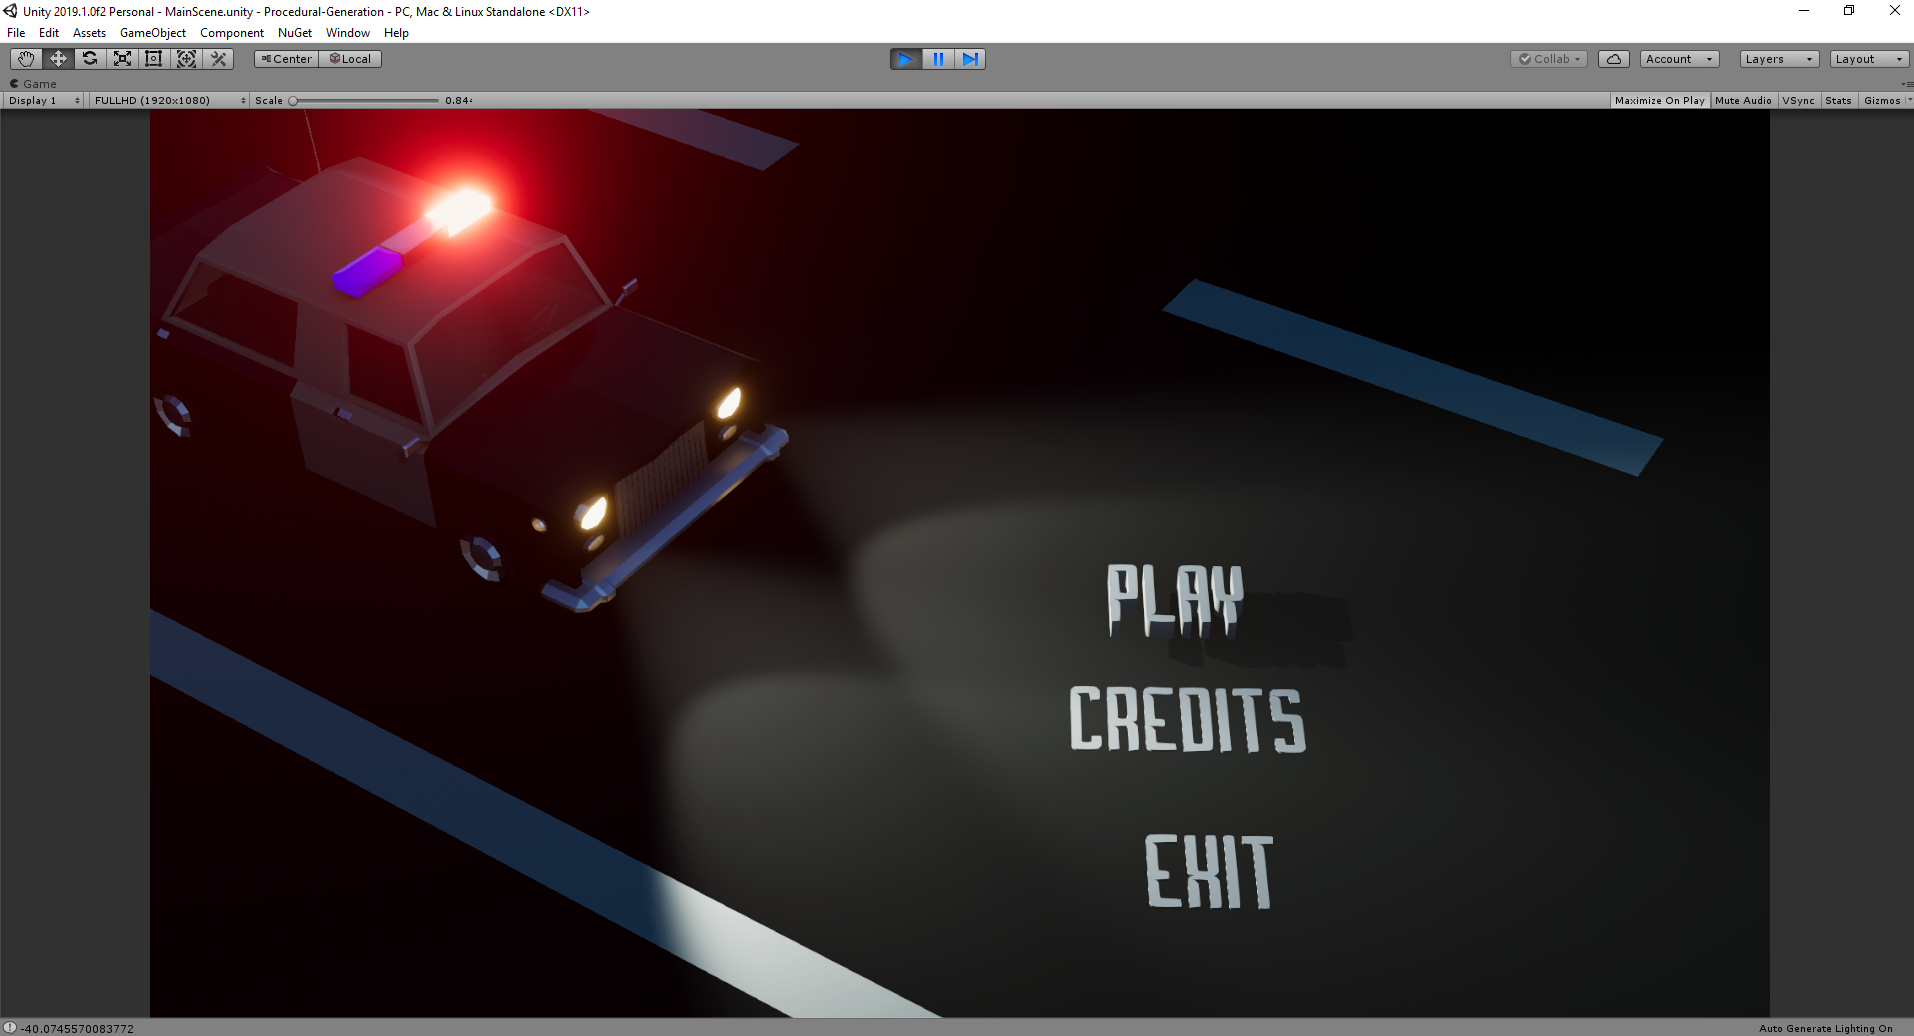
\includegraphics[width=\linewidth]{Meniu.png} \par
\caption{Meniul principal din joc}
\end{figure}

\vspace{10mm}
\begin{figure}[H]
\centering
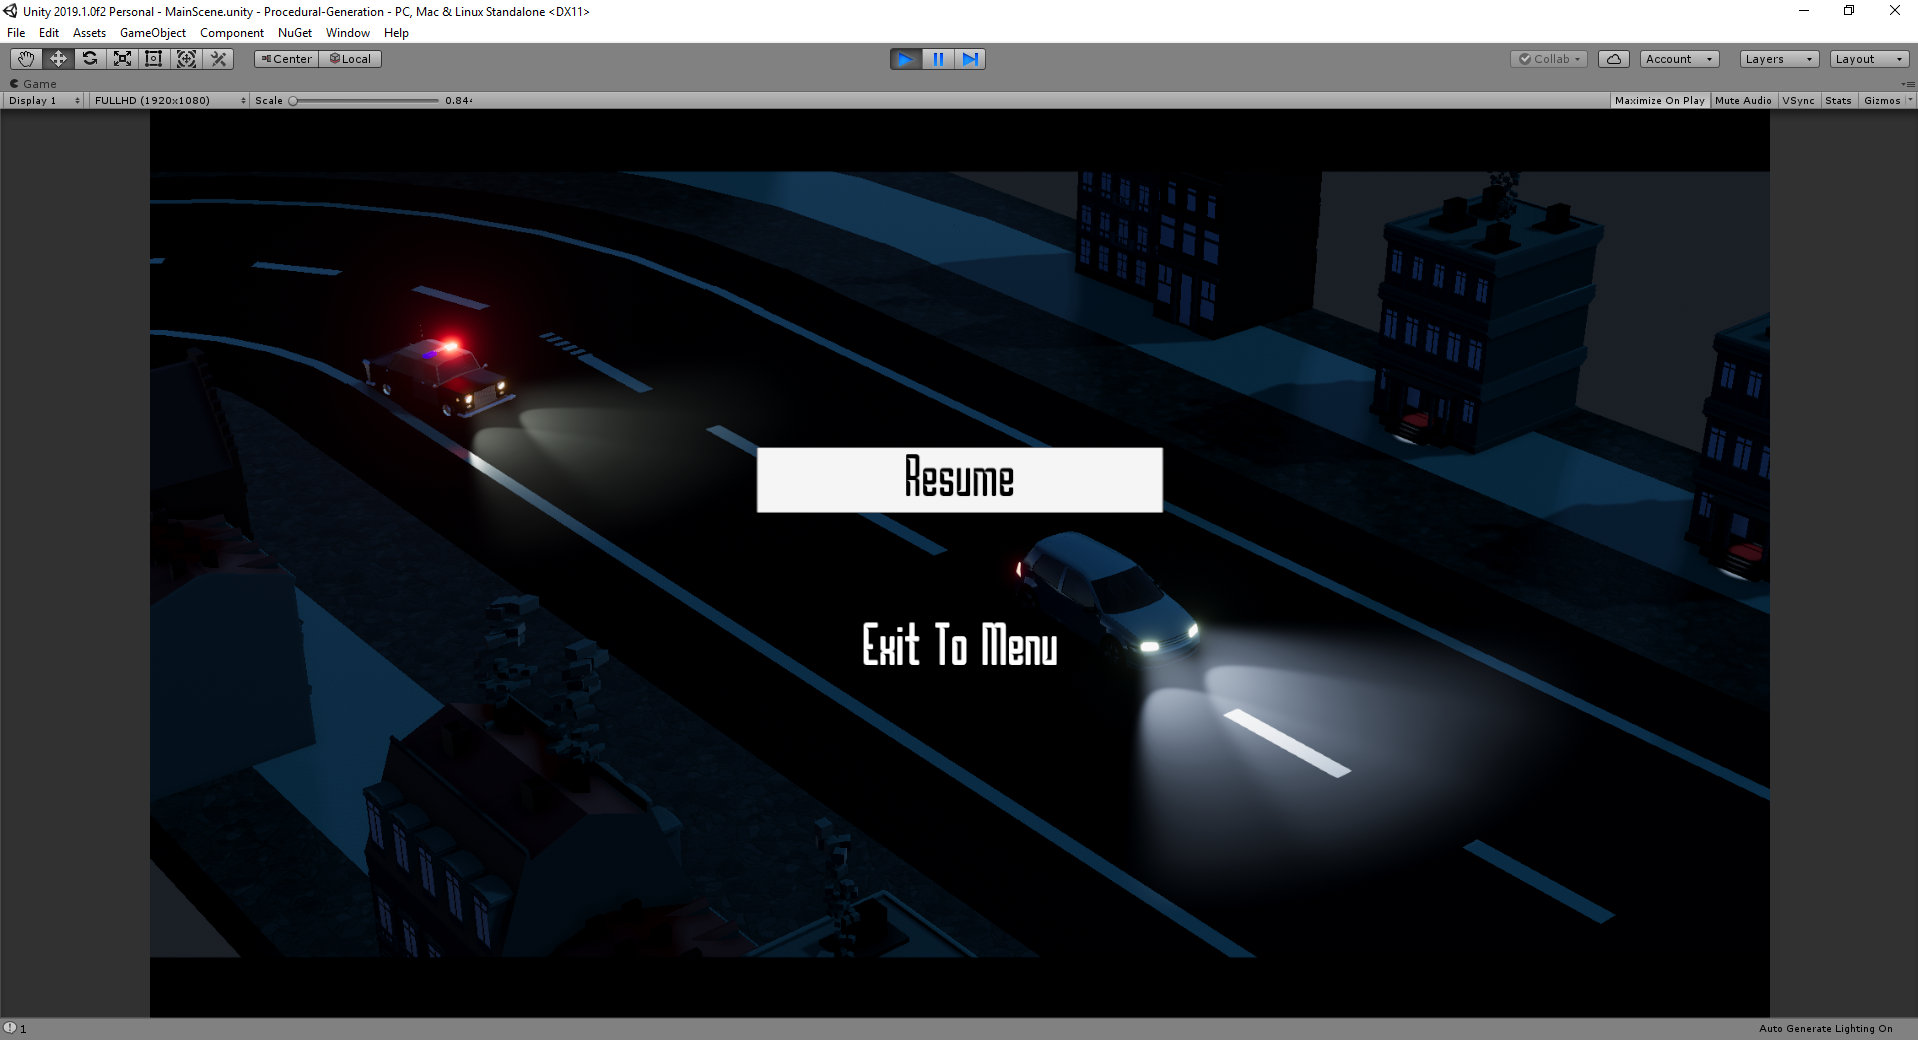
\includegraphics[width=\linewidth]{Pause.png} \par
\caption{Meniul de pauza}
\end{figure}

\vspace{10mm}
\begin{figure}[H]
\centering
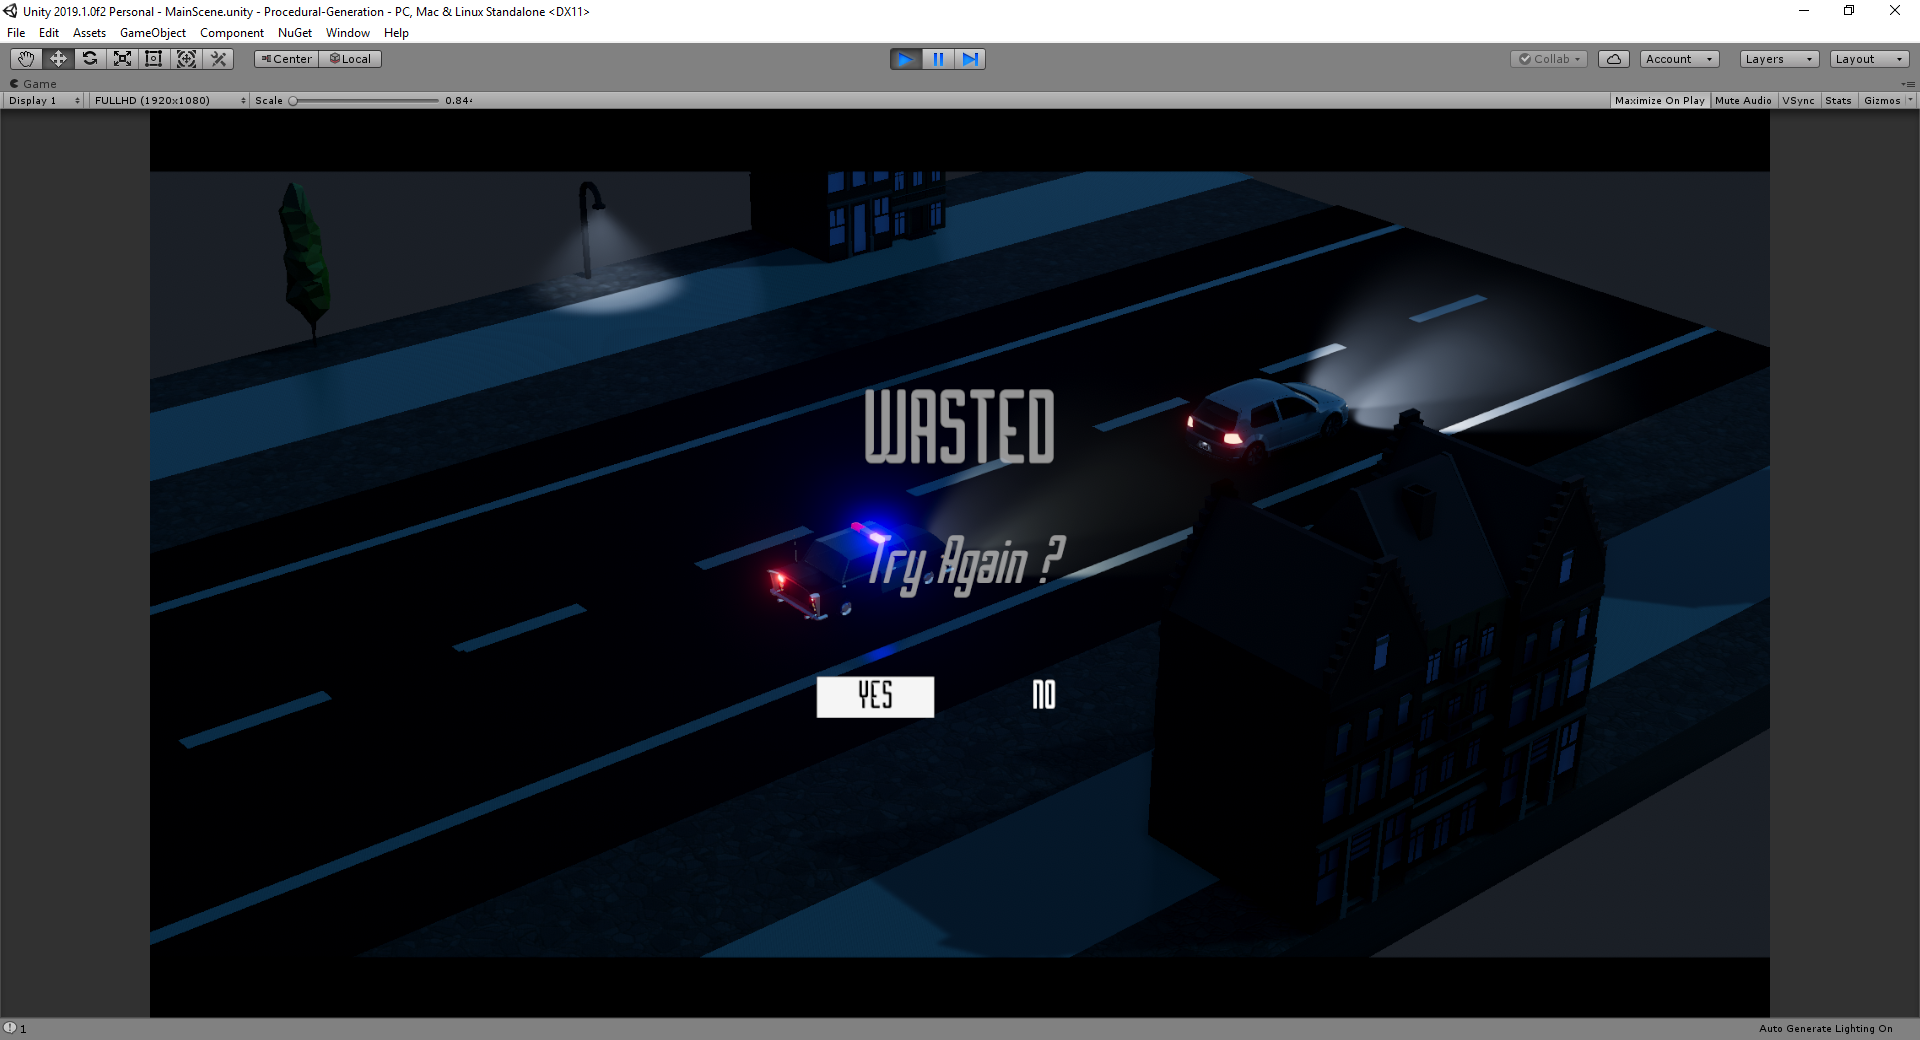
\includegraphics[width=\linewidth]{GameOver.png} \par
\caption{Meniul atunci cănd jocul s-a terminat}
\end{figure}

\section{Structura întregii aplicații}